\documentclass[11pt]{article}

\usepackage[margin=2.5cm]{geometry}
\usepackage{graphicx}
\usepackage{float}
\usepackage{graphicx}
\restylefloat{figure}

\title{Your Title}
\author{Your Name}
\date{\today}


\begin{document}

\maketitle
\pagebreak

\section{Introduction}
An arithmetic logic unit (ALU) is a multi-operation, combinational-logic digital function. It can 
perform a set of basic arithmetic operations and a set of logic operations. The ALU has a number of selection lines to select a particular operation in the unit. The selection lines are decoded 
within the ALU so that k selection variables can specify up to $2^k$
distinct operations.


Figure 1 shows the block diagram of a 4-bit ALU. The four data inputs from A are combined with the four inputs from B to generate an operation at the F outputs. The mode-select 
input $s_2$ distinguishes between arithmetic and logic operations. The two function-select inputs $s_1$
and $s_0$ specify the particular arithmetic or logic operation to be generated. With three selection 
variables, it is possible to specify four arithmetic operations (with $s_2$ in one state) and four logic 
operations (with $s_2$ in the other state). The input and output carries have meaning only during an 
arithmetic operation.
The input carry in the least significant position of an ALU is quite often used as a fourth 
selection variable that can double the number of arithmetic operations. In this way, it is possible 
to generate four more operations, for a total of eight arithmetic operations.

The input carry in the least significant position of an ALU is quite often used as a fourth 
selection variable that can double the number of arithmetic operations. In this way, it is possible 
to generate four more operations, for a total of eight arithmetic operations.

\begin{figure}[ht]
\centering
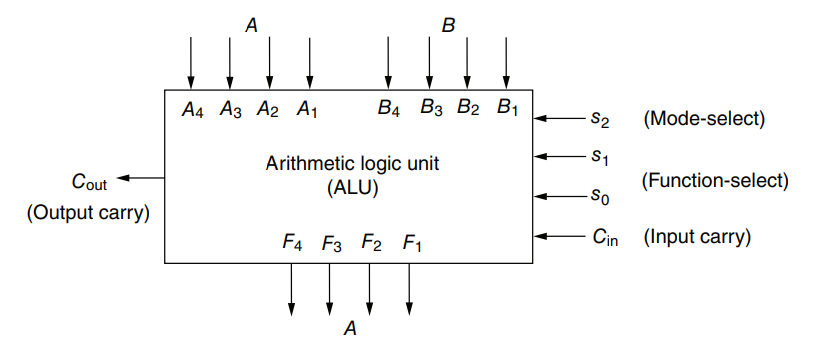
\includegraphics[width=0.9\textwidth]{images/ALU.png}
\caption{Block Diagram of a 4-bit ALU}
\end{figure}

The design of a typical ALU will be carried out in three stages. First, the design of the 
arithmetic section will be undertaken. Second, the design of the logic section will be considered. 
Finally, the arithmetic section will be modified so that it can perform both arithmetic and logic 
operations.

\section{Problem Specification with assigned instructions}
\textbf{Problem Specification:}
\begin{enumerate}
    \item Efficiently design (with minimum possible ICs) the ALU according to the specification.
    \item Implement the following flags:
    \begin{itemize}
        \item Carry (C)
        \item Sign (S)
        \item Overflow (V)
        \item Zero (Z)
    \end{itemize}
    \item Flags should be affected as per the rules of Assembly Language (with some exceptions).
    \item However, some exceptions (only for this assignment) has been added to incorporate 
    flexibility to flag status bits after logical operations. This flexibility is to 
    make the assignment easier, although it breaks some of the rules of the assembly 
    programming language.
    \begin{itemize}
        \item For NOT Operation:
            \begin{enumerate}
                \item After the NOT operation, Z flag is 1 if the answer is 0000 and the Z flag is 
                0 otherwise; ie. The Z flag functions as it normally would.
                \item After the NOT operation, if S remains unchanged or it reflects the highest 
                order bit of the result, both will be accepted. But if the S flag is changed and 
                it is changed to a wrong value, it will not be accepted.
                \item To make your life easier, we shall not check the C and V flags after NOT 
                operation, i.e., you can consider these as Don’t care.                
            \end{enumerate}
        \item For AND/OR/XOR Operation:
            \begin{enumerate}
                \item C and V should be cleared (0) after the operation.
                \item S and Z should be changed according to the output.
            \end{enumerate}
    \end{itemize}
    \item Any 2-input SSI (AND, OR, NOT, XOR, etc.) and MSI (MUX, Decoder, Adder, etc.) 
    chip can be used.
    \item Emphasis should be given to the efficiency of design and minimization of ICs used.
    \item For simulation, one can use any simulation software.
    \item Software design must be at IC level.
    \item Everyone have to write a report.
\end{enumerate}
\textbf{Functional Design Specifications:}

\begin{table}[ht]
    \centering
    \begin{tabular}{|c|c|c|c|}
        \hline
        \textbf{CS2} & \textbf{CS1} & \textbf{CS0} & \textbf{Functions} \\
        \hline
        0 & 0 & 0 & Add \\
        \hline
        0 & 0 & 1 & AND \\
        \hline
        0 & 1 & X & Sub with borrow \\
        \hline
        1 & 0 & 0 & Complement A \\
        \hline
        1 & 0 & 1 & OR \\
        \hline
        1 & 1 & X & NEG A \\
        \hline
    \end{tabular}
    \caption{Control Signals and Functions of the 4-bit ALU}
\end{table}

Here, CS2, CS1, and CS0 are the control signals. X means that the value of the signal is not important.
\begin{figure}[ht]
    \centering
    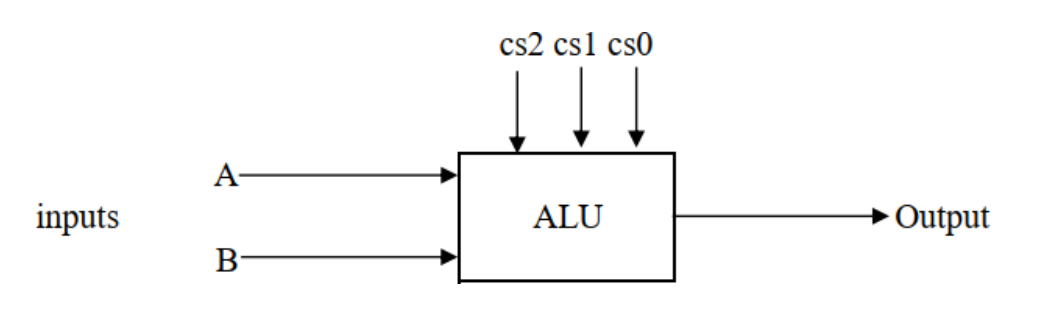
\includegraphics[width=0.9\textwidth]{images/ALU2.png}
    \caption{Block Diagram of a 4-bit ALU}
\end{figure}

\section{Detailed design steps with k-maps (if applicable)}

\section{Truth Table}
\begin{table}[ht]
    \centering
    \begin{tabular}{|c|c|c|c|c|c|c|c|c|c|c|}
        \hline
        CS2 & CS1 & CS0 & Functions & X & S11 & S10 & Y & $\bar{\textnormal{E2}}$ & S2 & Cin \\
        \hline
        0 & 0 & 0 & Add & A & 0 & 0 & B & 0 & 0 & 0 \\
        \hline
        0 & 0 & 1 & AND & AB & 0 & 1 & 0 & 1 & X & 0 \\
        \hline
        0 & 1 & X & Sub with borrow & A & 0 & 0 & B' & 0 & 1 & 0 \\
        \hline
        1 & 0 & 0 & Complement A & A' & 1 & 0 & 0 & 1 & X & 0 \\
        \hline
        1 & 0 & 1 & OR & A+B & 1 & 1 & 0 & 1 & X & 0 \\
        \hline
        1 & 1 & X & NEG A & A' & 1 & 0 & 0 & 1 & X & 1 \\
        \hline
    \end{tabular}
    \caption{Truth Table of the 4-bit ALU}
\end{table}

\section{Block Diagram}

\section{Complete Circuit Diagram}

\section{ICs used with count as a chart}
\begin{table}[ht]
    \centering
    \begin{tabular}{|c|c|}
        \hline
        IC & Count \\
        \hline
        74153 & 2 \\
        \hline
        74157 & 1 \\
        \hline
        7408 & 2 \\
        \hline
        7432 & 2 \\
        \hline
        7404 & 2 \\
        \hline
        7486 & 1 \\
        \hline
        7483 & 2 \\
        \hline
    \end{tabular}
\end{table}

\section{The simulator used along with the version number}

\section{Discussions}

\section{Contribution of Each Member}

\end{document}
